%!TeX root = main.tex

\begin{frame}{\insertsection}
	\begin{figure}
		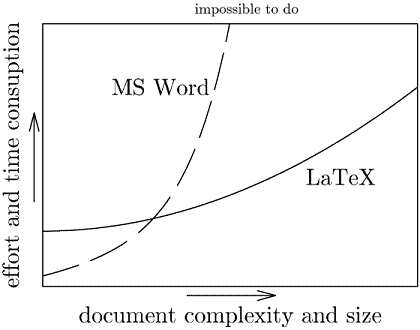
\includegraphics[scale=0.5]{./Images/latex-difficulty-2.png}
	\end{figure}
\end{frame}

\begin{frame}{\insertsection}{Work flow improvements}
	\begin{figure}
		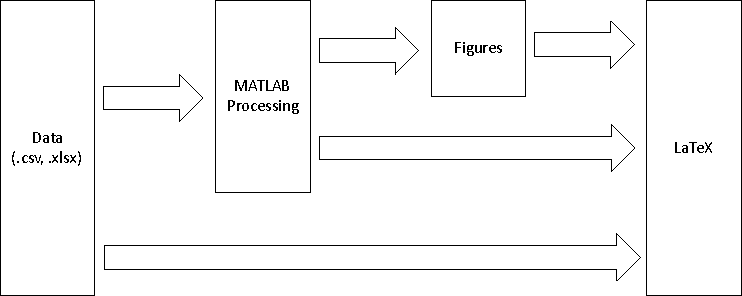
\includegraphics[width=0.7\linewidth]{./Images/workflow.pdf}
	\end{figure}
\end{frame}

\begin{frame}{\insertsection}{Pretty Pictures}
	\begin{figure}
		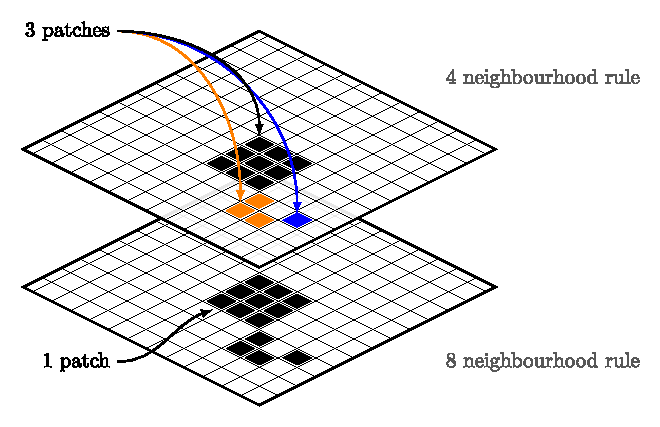
\includegraphics[width=0.35\linewidth]{./Images/Neighbourhood_definition2.pdf}
		\hspace{5em}
		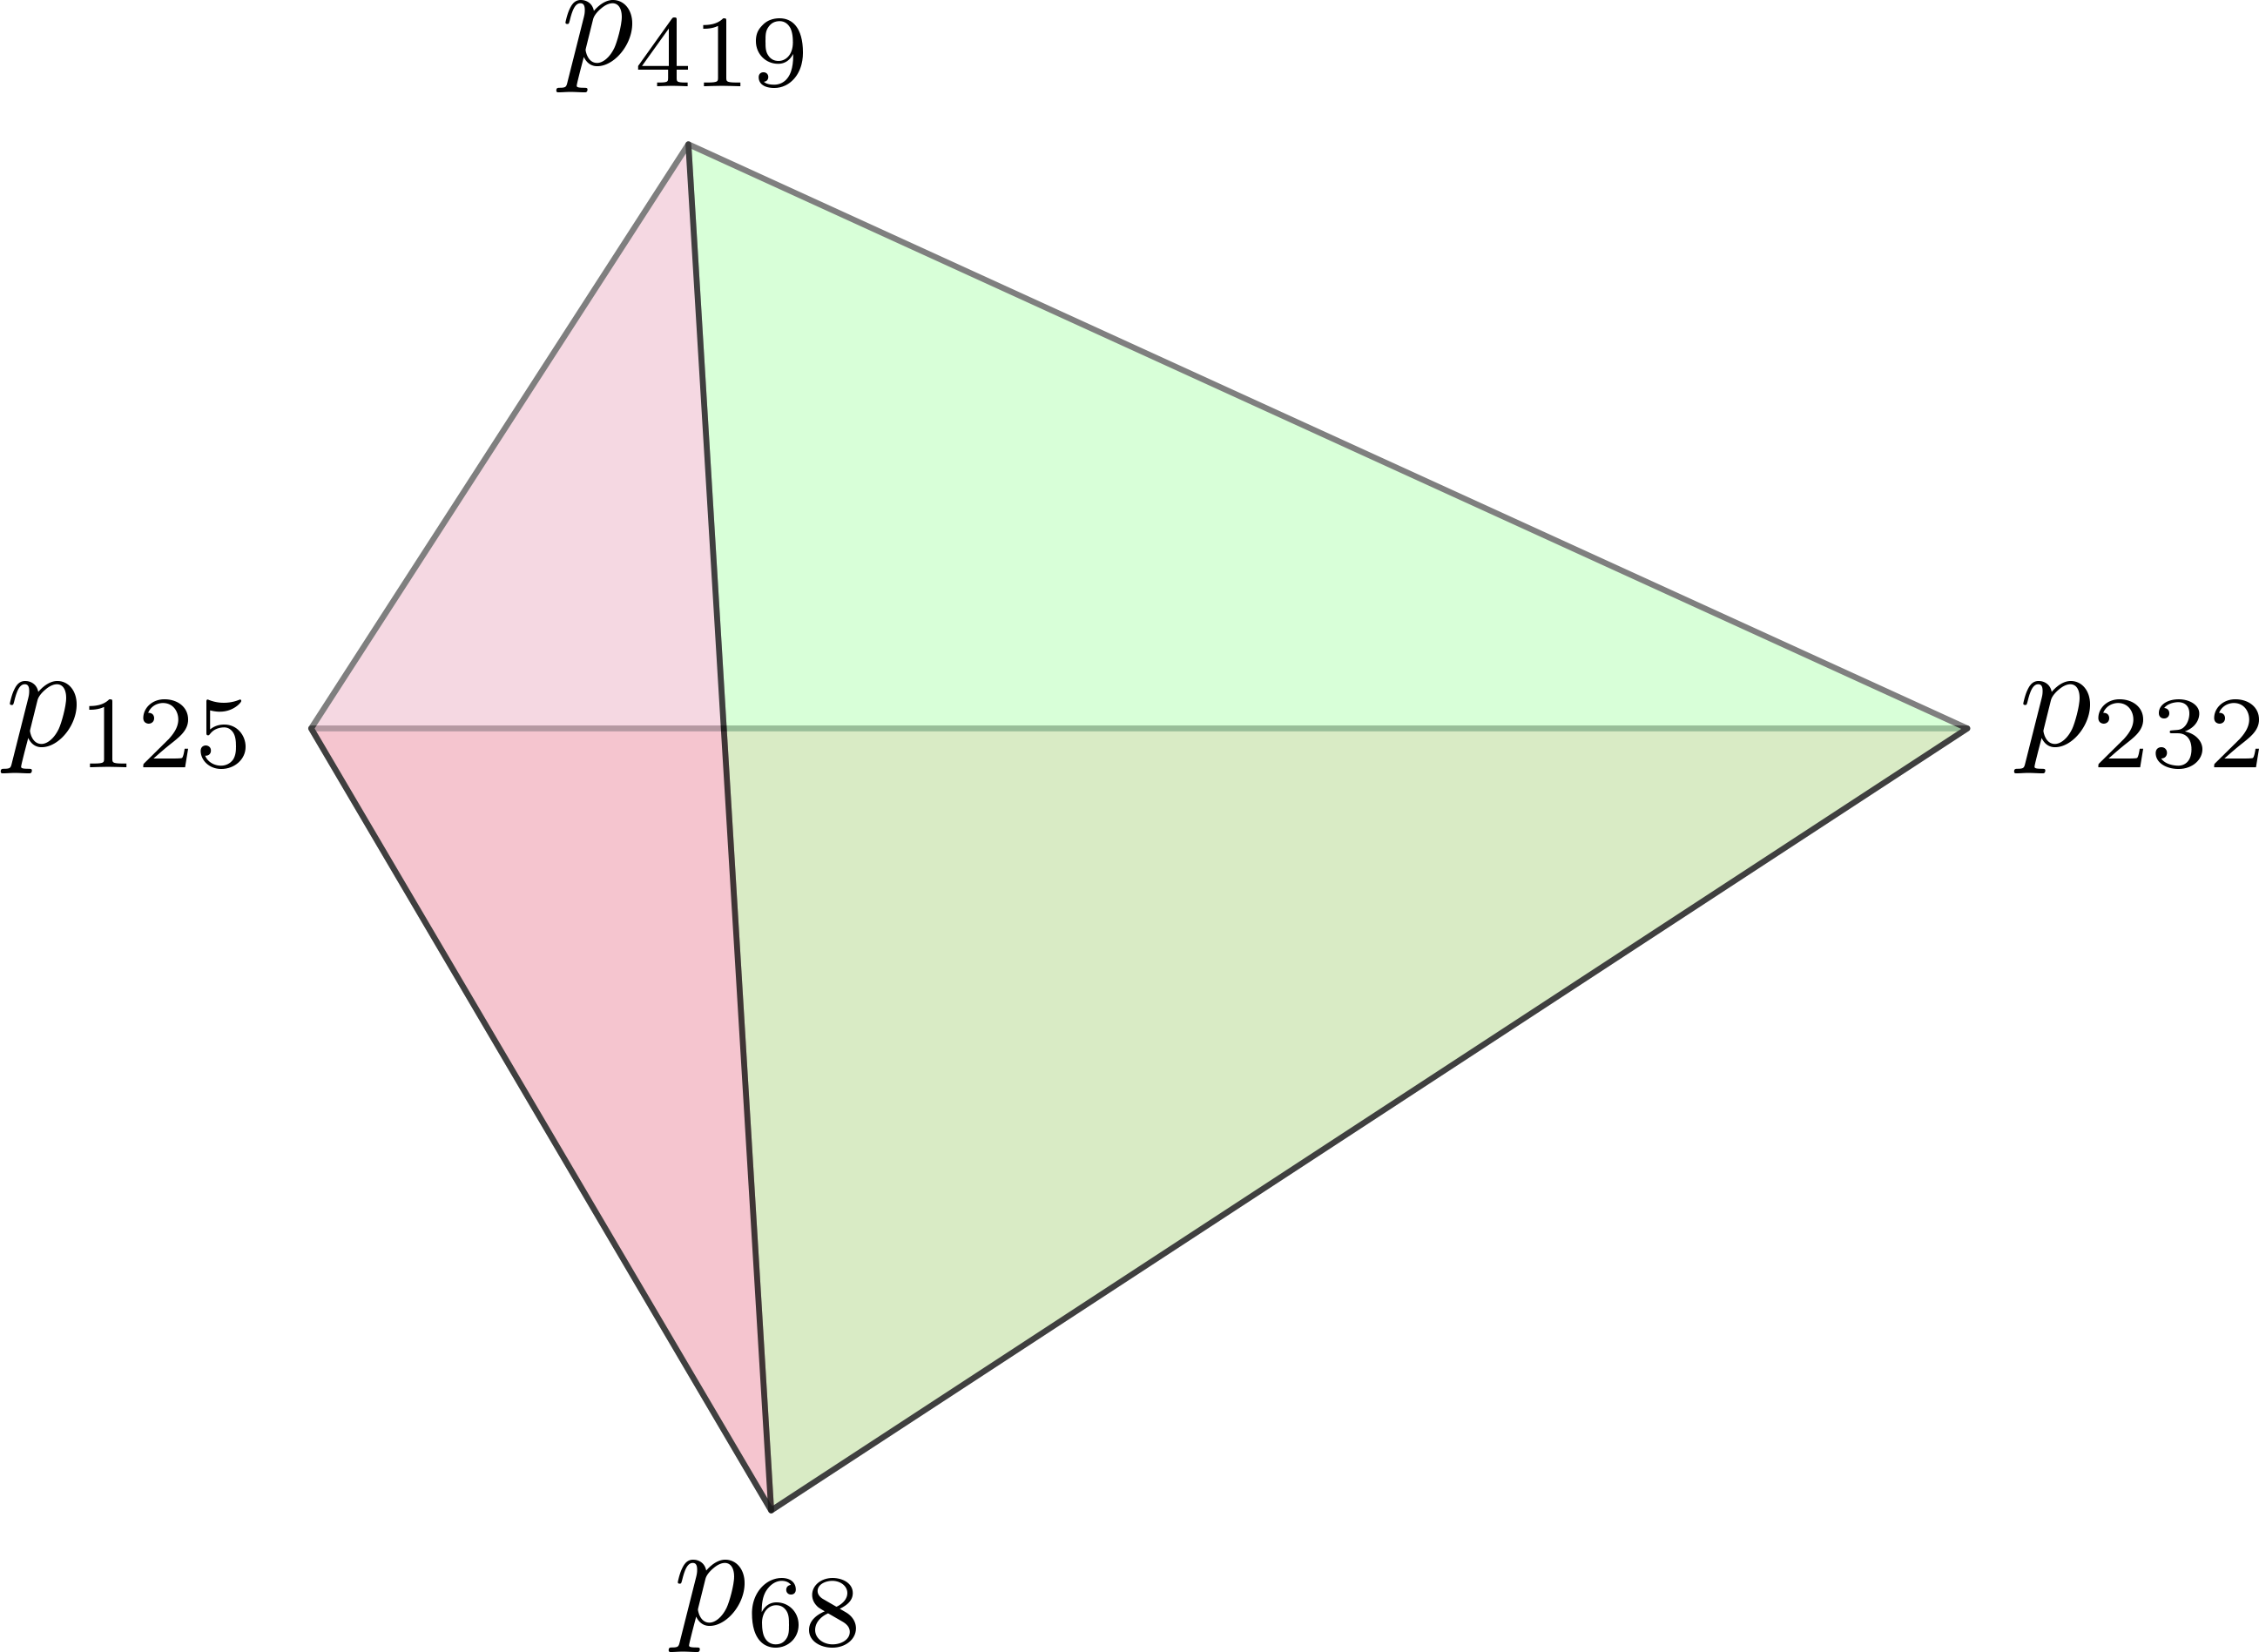
\includegraphics[width=0.35\linewidth]{./Images/nicePic.png}
	\end{figure}
	\blfootnote{PGF -- \url{https://ctan.org/pkg/pgf?lang=en}}
\end{frame}

\begin{frame}{\insertsection}{Circuitry}
	\begin{figure}
		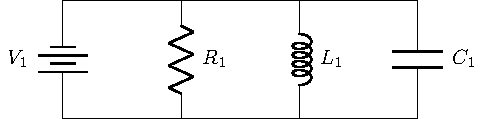
\includegraphics[width=0.7\linewidth]{./LaTex_Tikz/circuitikz.pdf}
	\end{figure}
	\blfootnote{circuitikz -- \url{https://ctan.org/pkg/circuitikz?lang=en}}
\end{frame}

\begin{frame}{\insertsection}{Presentation}
	\begin{figure}
		
\includegraphics[width=0.4\linewidth]{./Images/beamer.png}
	\end{figure}
	\blfootnote{Beamer Class -- \url{https://ctan.org/pkg/beamer?lang=en}}
\end{frame}

\begin{frame}{\insertsection}{Exams}
	\begin{figure}
		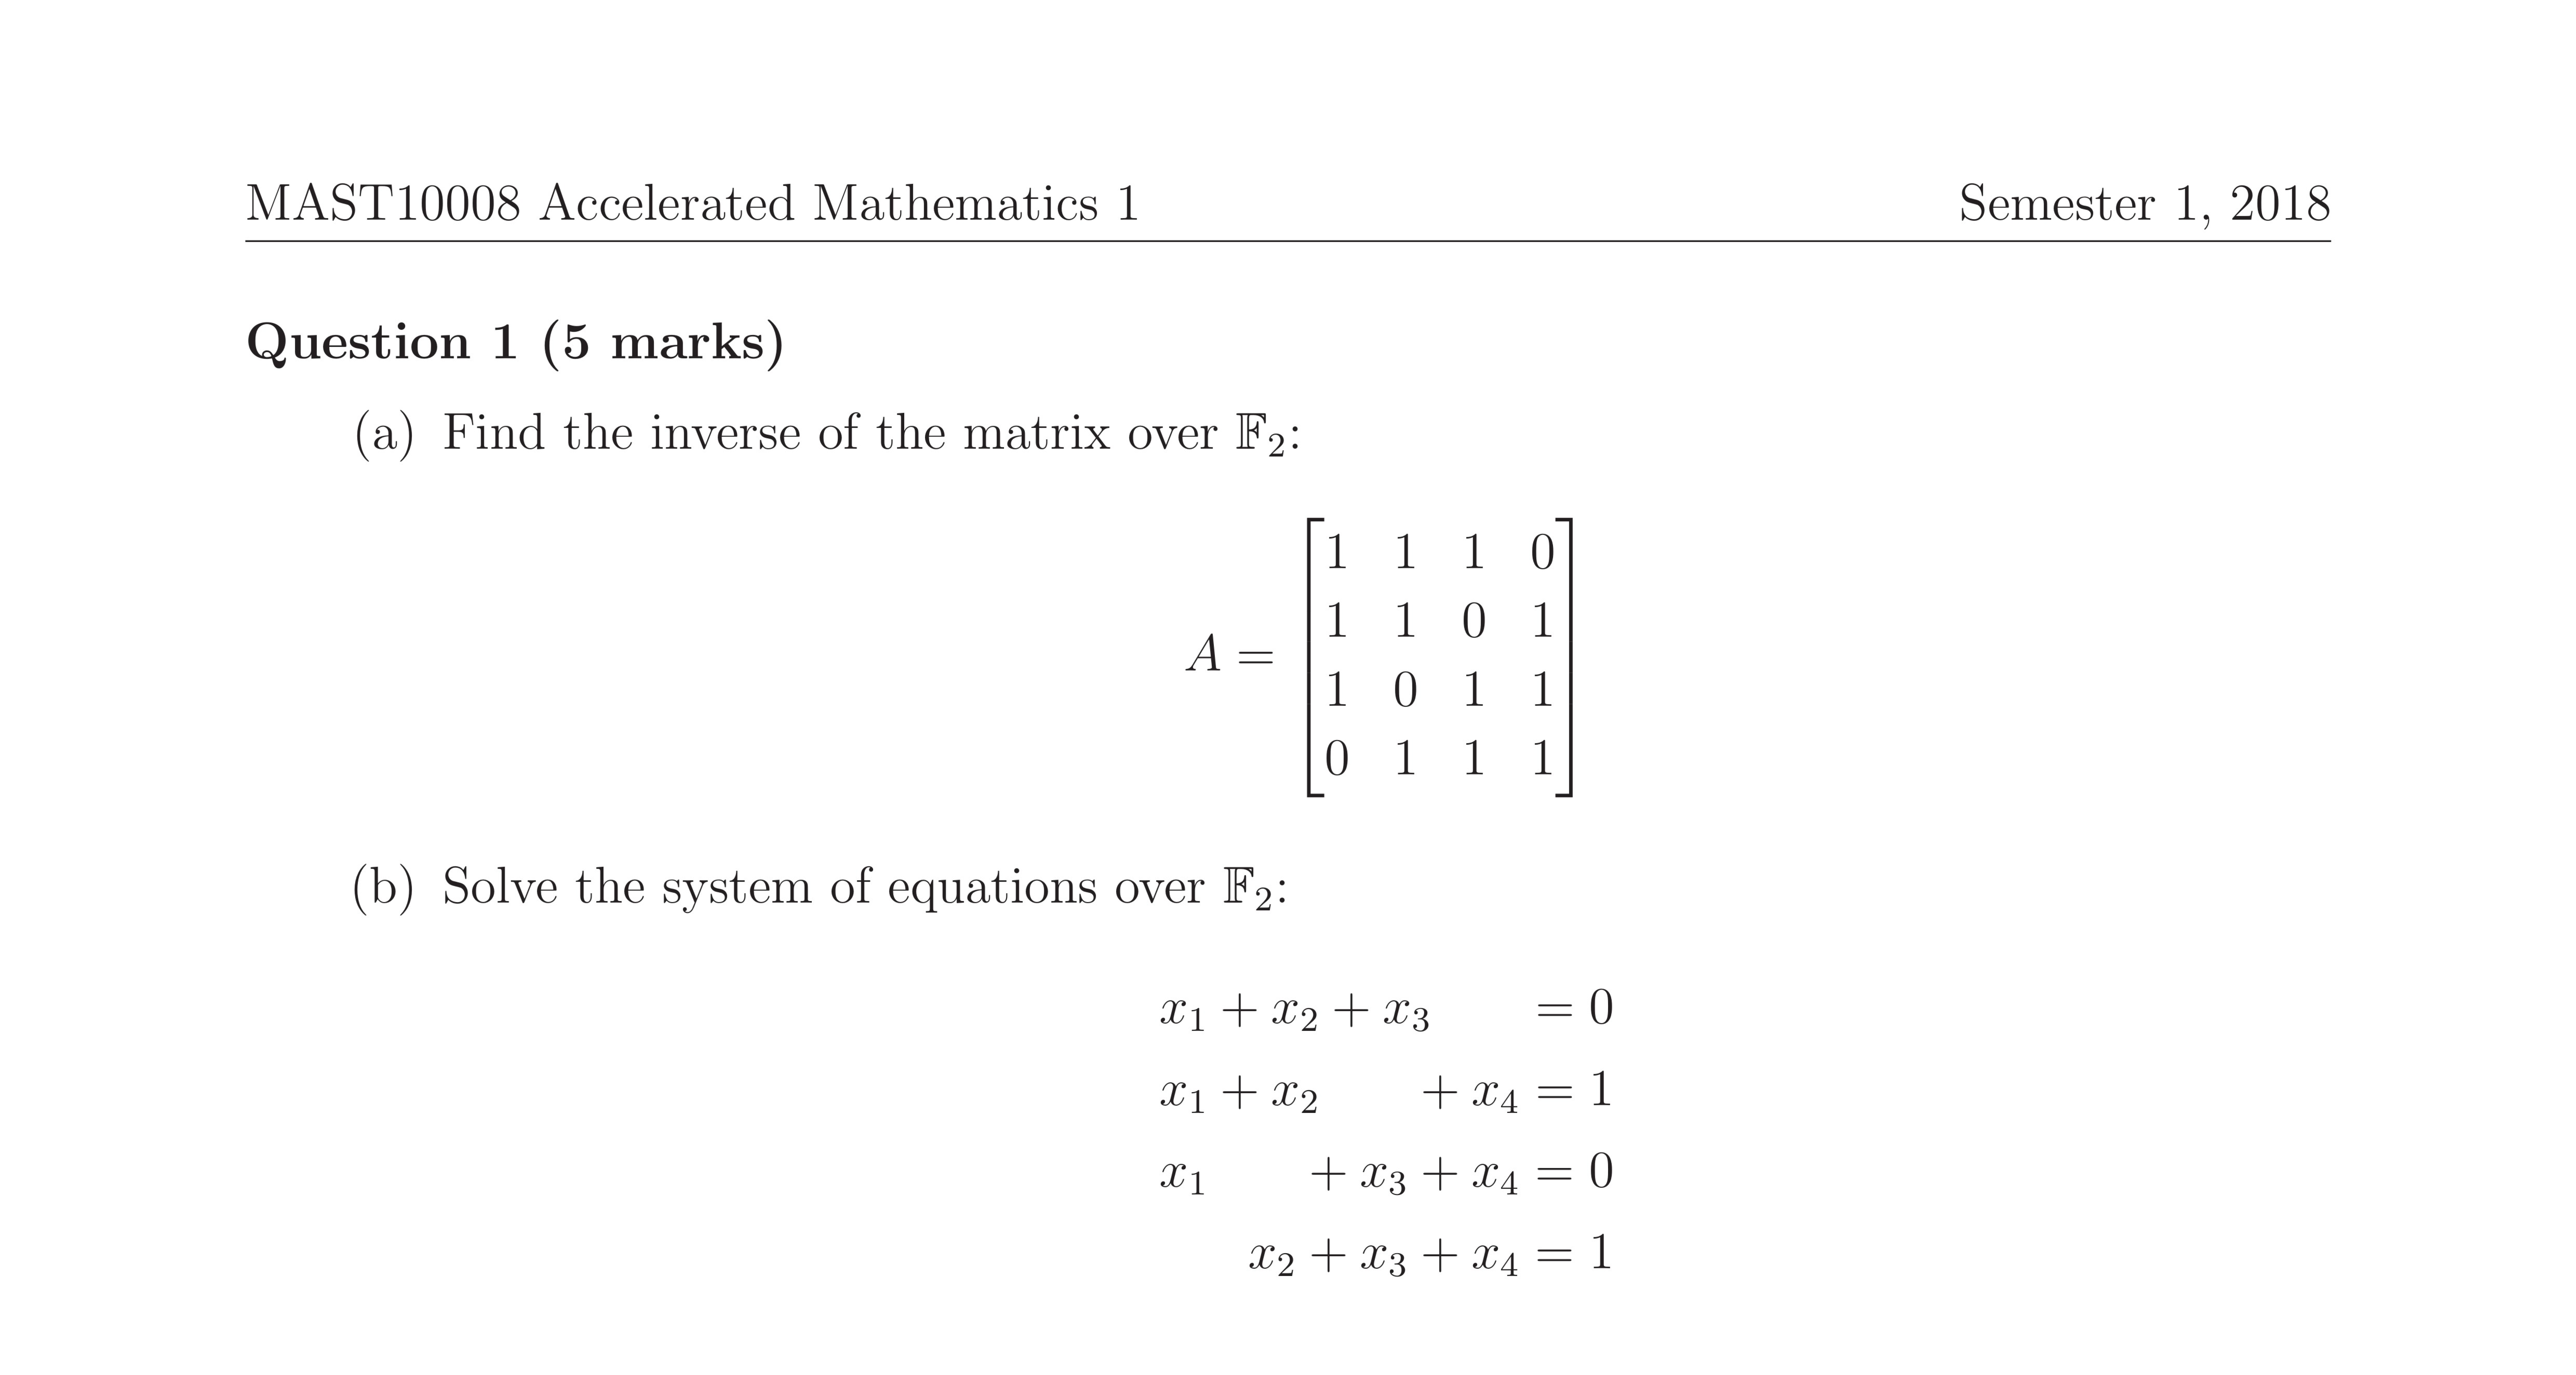
\includegraphics[width=0.4\linewidth]{./Images/AM1-2.png}
		\hspace{5em}
		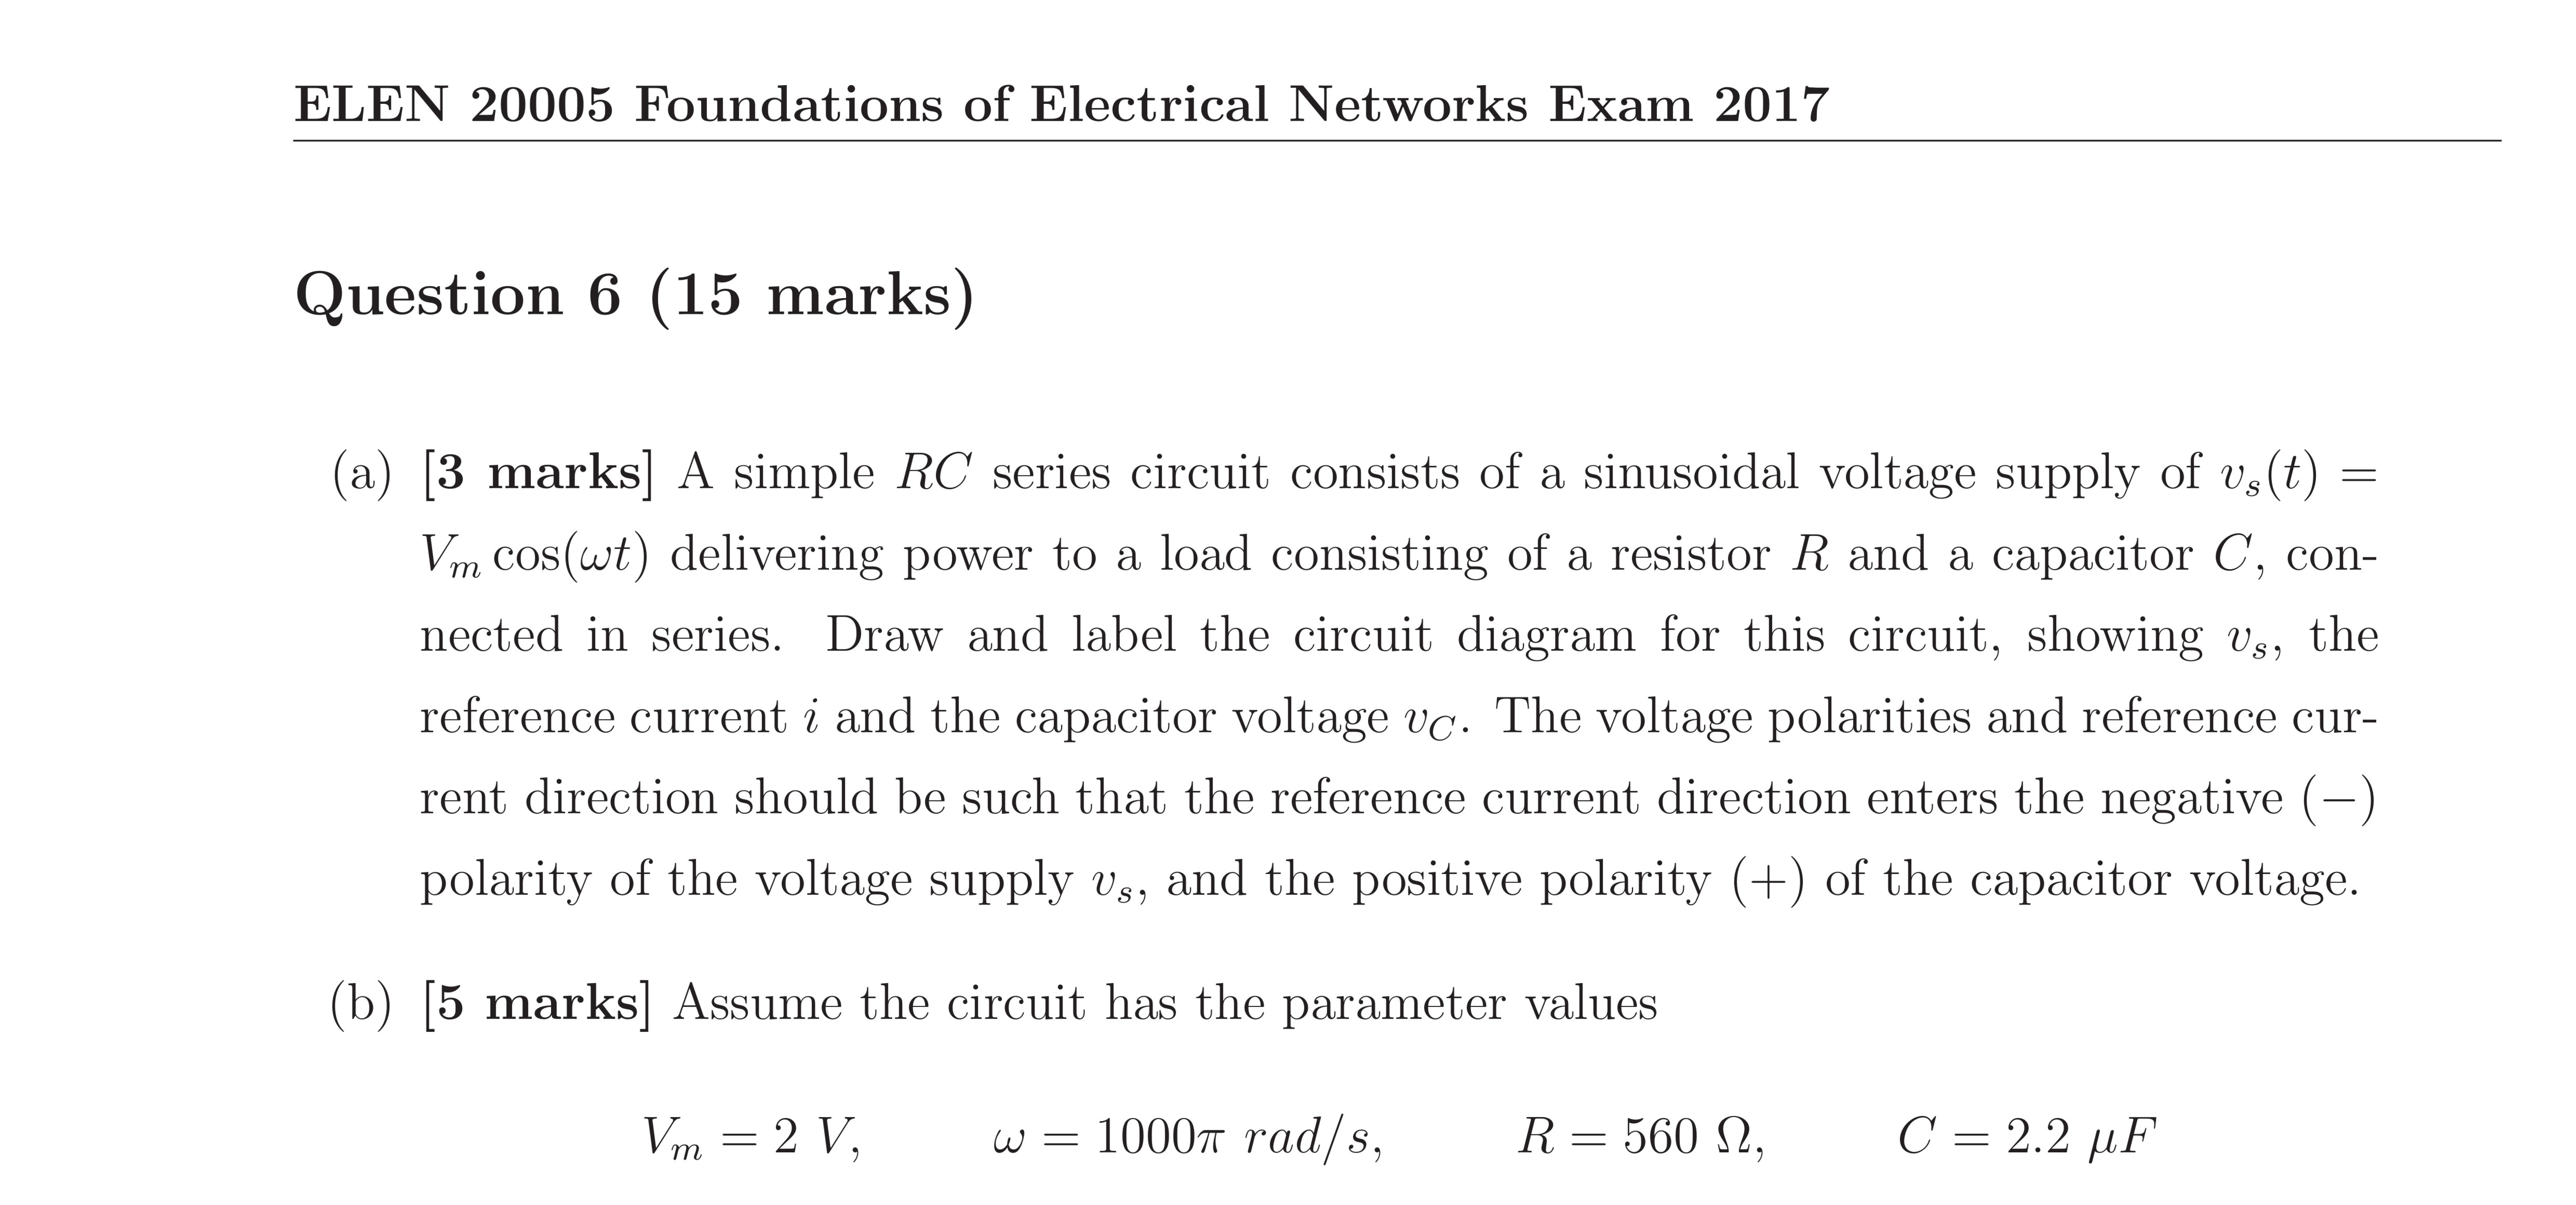
\includegraphics[width=0.4\linewidth]{./Images/elen.png}
	\end{figure}
	\blfootnote{Exam Class -- \url{https://ctan.org/pkg/exam?lang=en}}
\end{frame}

\begin{frame}{\insertsection}{Code Highlighting}
	\tiny{\inputminted[numbers=none, frame=single]{matlab}{./Example_Codes/A_over_Astar_isentropic.m}}
	\blfootnote{Exam Class -- \url{https://ctan.org/pkg/exam?lang=en}}
\end{frame}

\begin{frame}{\insertsection}{}
	\centering
	\Huge{Most Importantly}
\end{frame}

\begin{frame}{\insertsection}{Academically Professional}
	\begin{figure}
		
\includegraphics[height=0.7\textheight]{./Images/file_extensions_2x.png}
		\hspace{5em}
		
\includegraphics[height=0.7\textheight]{./Images/latex.png}
	\end{figure}
\end{frame}